\documentclass[12pt,letterpaper]{article}
\usepackage[utf8]{inputenc}
\usepackage[margin=1in]{geometry}
\usepackage{graphicx}
\usepackage{titling}
\usepackage{amsmath}
\usepackage{amsfonts}
\usepackage{amssymb}
\renewcommand{\theenumiv}{\arabic{enumiv}}
\setlength{\droptitle}{-5em}
\author{Maurice Diesendruck}
\title{StatMod2 - Gibbs - Exercises 4}
\begin{document}
\maketitle

\section{Gibbs Sampler}
\subsection{Model}

\begin{align*}
	y &\sim\ N(X\pmb{\beta}, \sigma^2\pmb{I})\\
	\beta|\tau^2 \sim\ N(\pmb{0, \tau^2\pmb{I})\\
	\sigma^2 &\sim\ IG(a/2, b/2)\\
	\tau^2 &\sim\ IG(c/2, d/2)
\end{align*}




\newpage

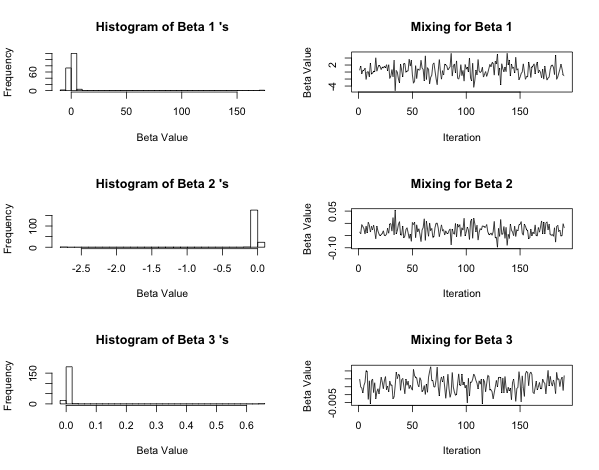
\includegraphics[width=150mm,scale=1.5]{hw32pic.png}

\end{document}
